\section{Background}
Energy consumption is ever increasing, and our current power-line network is outdated, as it allows only for very limited variations in pricing (either fixed-price or very low segmentation of the 24-hour day).
However, there is also an increasing generation of renewable energy (e.g. wind and solar energy), but optimal use of this is limited by the current power-grid, as availability is very fluctuating.
This is why there now is a focus on energy usage, with optimizations of the power-grid as a high priority, which is why by 2022 all\footnote{80\% by 2020} electrical meters in EU member countries will have been replaced by \textit{smart meters} \cite{smart_meter_survey} \cite{directive_2009_72_EC}.
An expansion of the power-line grid, as it is extended to connect more EU member countries, along with the addition of smart meters -- enabling home owners to supply themselves and others, will form a smart grid.

\subsection{Smart Grid and Smart Meters}
A smart grid is a power-line grid expanded by a net, allowing two-way communication, where it was earlier one-way.
This allows for much more dynamic power supply and consumption, as suppliers will know more about their consumers, and consumers will have more options in regards to their consumption.
The outline of a smart grid can be seen in \cref{fig:background:smartgrid}.
In the figure can be seen three main actors: power suppliers (Windmills, solar panels, traditional power plants, external suppliers), net supplier (Datahub -- Danish term from \cite{LOV_nr_575_af_18-06-2012}, smart meters), and end consumers (Smart home and buildings).

The smart grid serves several purposes \cite{smartgrid_gov} \cite{directive_2009_72_EC}:
\begin{itemize}
	\item Adjusting prices based on supply and demand.
	\item Adjusting prices based on type of energy available, as renewable energy is less dependable, and often only more expensive energy is available.
	\item Easily change energy supplier, in order to increase market competitiveness.
	\item Connect power-lines across Europe, greater enabling the three points above.
	\item Allowing users to monitor their own energy usage.
	\item Allowing users to adjust their energy consumption based on available energy/prices.
	\item Allowing users to be suppliers to the smart grid.
	\item Allowing users to use smart appliances, connected to the smart meter, allowing for home automation and optimized energy usage.
\end{itemize}

\begin{figure}
	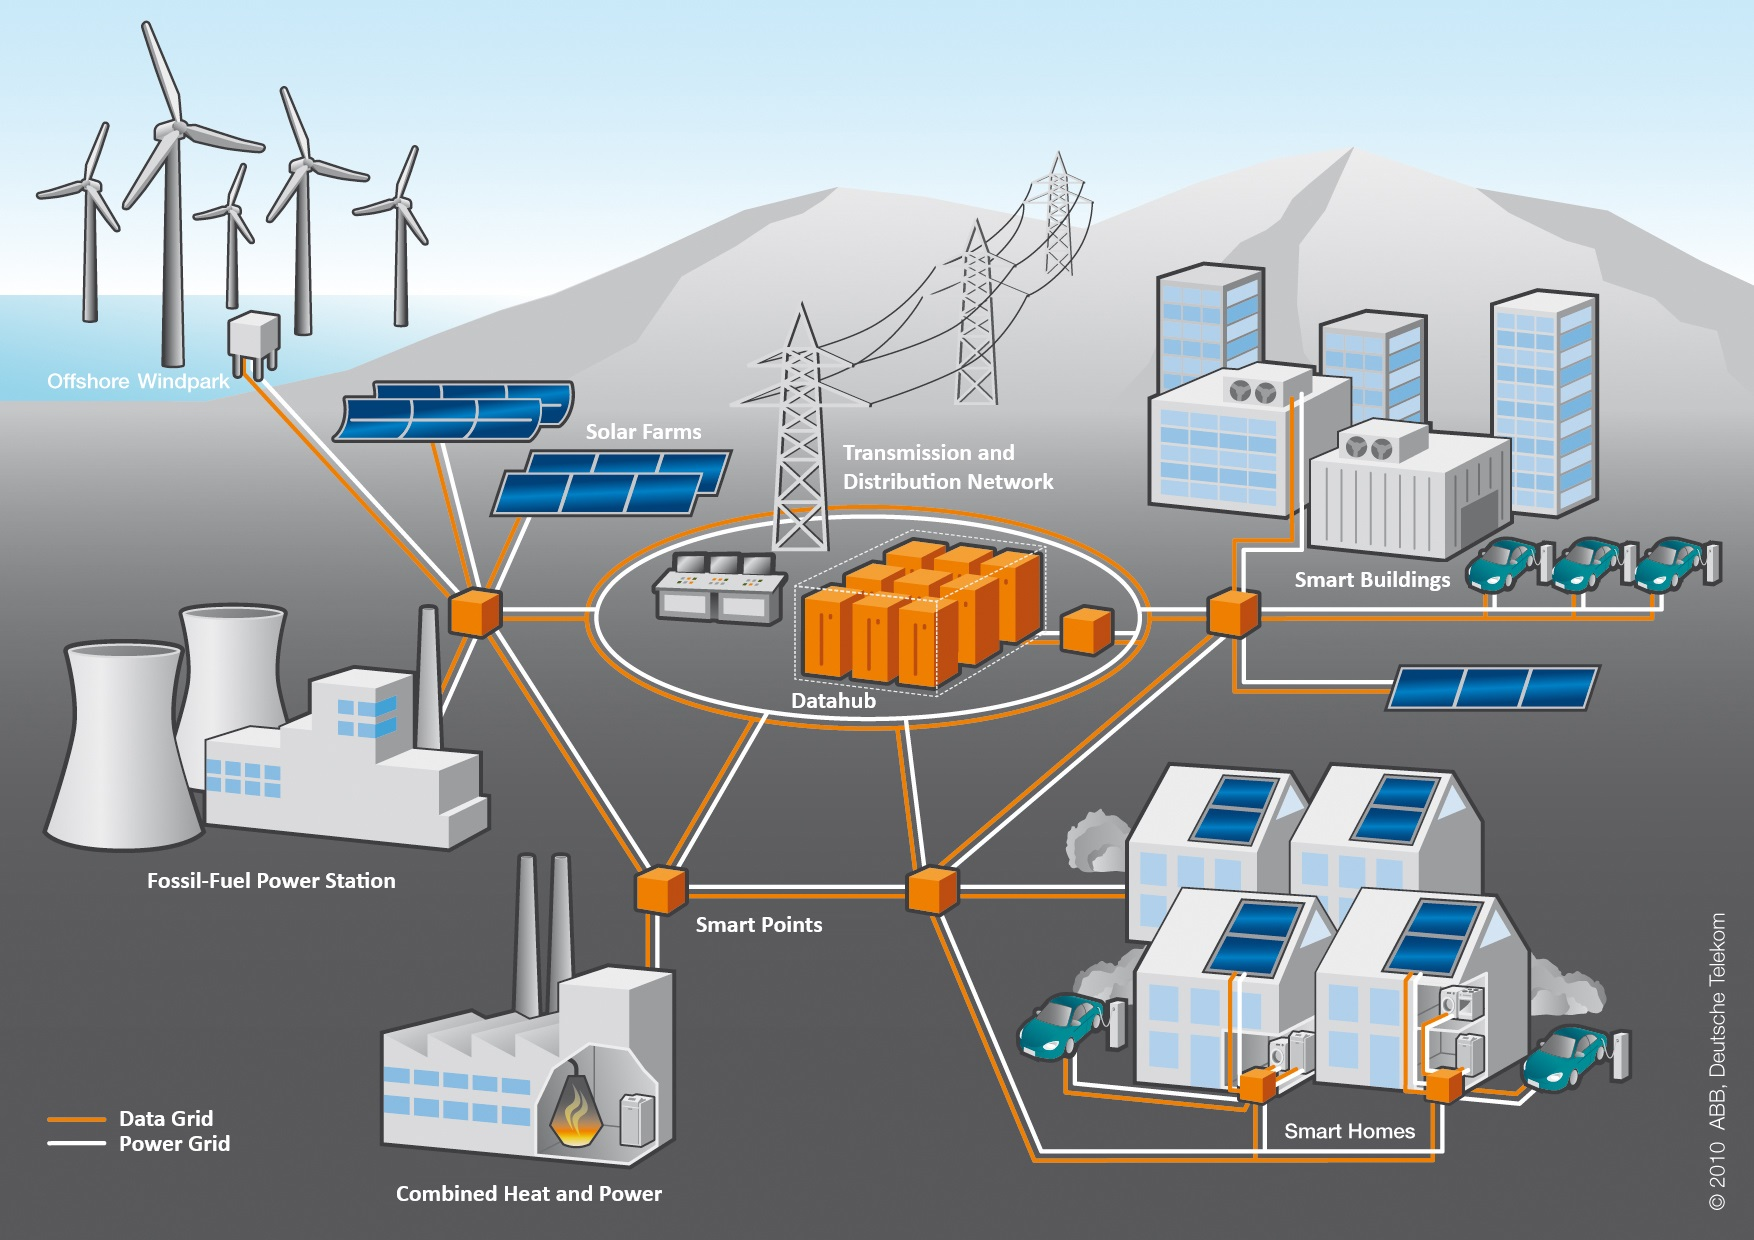
\includegraphics[width=\textwidth]{figures/SmartGrid_Ueberblick_ohneLegende.jpg}
	\caption{\url{http://powertown.no/wp-content/uploads/2011/11/SmartGrid_Ueberblick_ohneLegende.jpg} \url{https://www.telekom.com/medien/bild-ton-und-infografiken/infografiken/155030}}
	\label{fig:background:smartgrid}
\end{figure}

\subsection{Problems}
In regards to enabling an EU-wide smart grid, there are bound to be problems as this is an immense project.
This roll-out will not be the same in every nation, as each nation has its own infrastructure and differs in which parts of the current power-grid is owned/regulated by state and what is part of a free market.
However, some shared problems still exist, such as privacy, conflict of interest, and attack vulnerabilities \cite{offswitch} \cite{smart_meter_survey}.

\paragraph{Different architectures}

\paragraph{Privacy}

\paragraph{Conflict of interest}

\paragraph{Vulnerabilities}
